\documentclass{report}
\usepackage{listings}
\usepackage[dvipsnames]{xcolor}
\pagecolor{GreenYellow!10}
\usepackage[utf8]{inputenc}
\usepackage[spanish,mexico]{babel}
\setlength{\textwidth}{18cm}
\setlength{\oddsidemargin}{-1cm}
\setlength{\headsep}{-1cm}
\setlength{\voffset}{0cm}
\setlength{\topmargin}{0cm}
\setlength{\headheight}{0cm}
\usepackage{tikz}
\usetikzlibrary{calc,arrows}
\usepackage{multicol}
\usepackage{lipsum} 

%%%%%% LISTINGS %%%%%%%%%%%%%%%%%%%%%%%%%%%%%%%%%%%%%%%%%
\definecolor{codegreen}{rgb}{0,0.6,0}
\definecolor{codegray}{rgb}{0.5,0.5,0.5}
\definecolor{codepurple}{rgb}{0.58,0,0.82}
\definecolor{backcolour}{rgb}{8.9,8.9,0.9}
\lstdefinestyle{mystyle}{
    backgroundcolor=\color{backcolour},
	commentstyle=\color{codegreen},
	keywordstyle=\color{magenta},
    numberstyle=\tiny\color{codegray},
    stringstyle=\color{codepurple},
    basicstyle=\ttfamily\footnotesize,
    breakatwhitespace=false,         
    breaklines=true,                 
    captionpos=b,                    
    keepspaces=true,                 
    numbers=left,                    
    numbersep=5pt,                  
    showspaces=false,                
    showstringspaces=false,
    showtabs=false,                  
    tabsize=2
}

\lstset{style=mystyle}

\begin{document}
%%%%%% ENCABEZADO %%%%%%%%%%%%%%%%%%%%%%%%%%%%%%%%%%%%%%%
    \begin{minipage}[t]{0.165 \textwidth}
       \begin{flushright}
        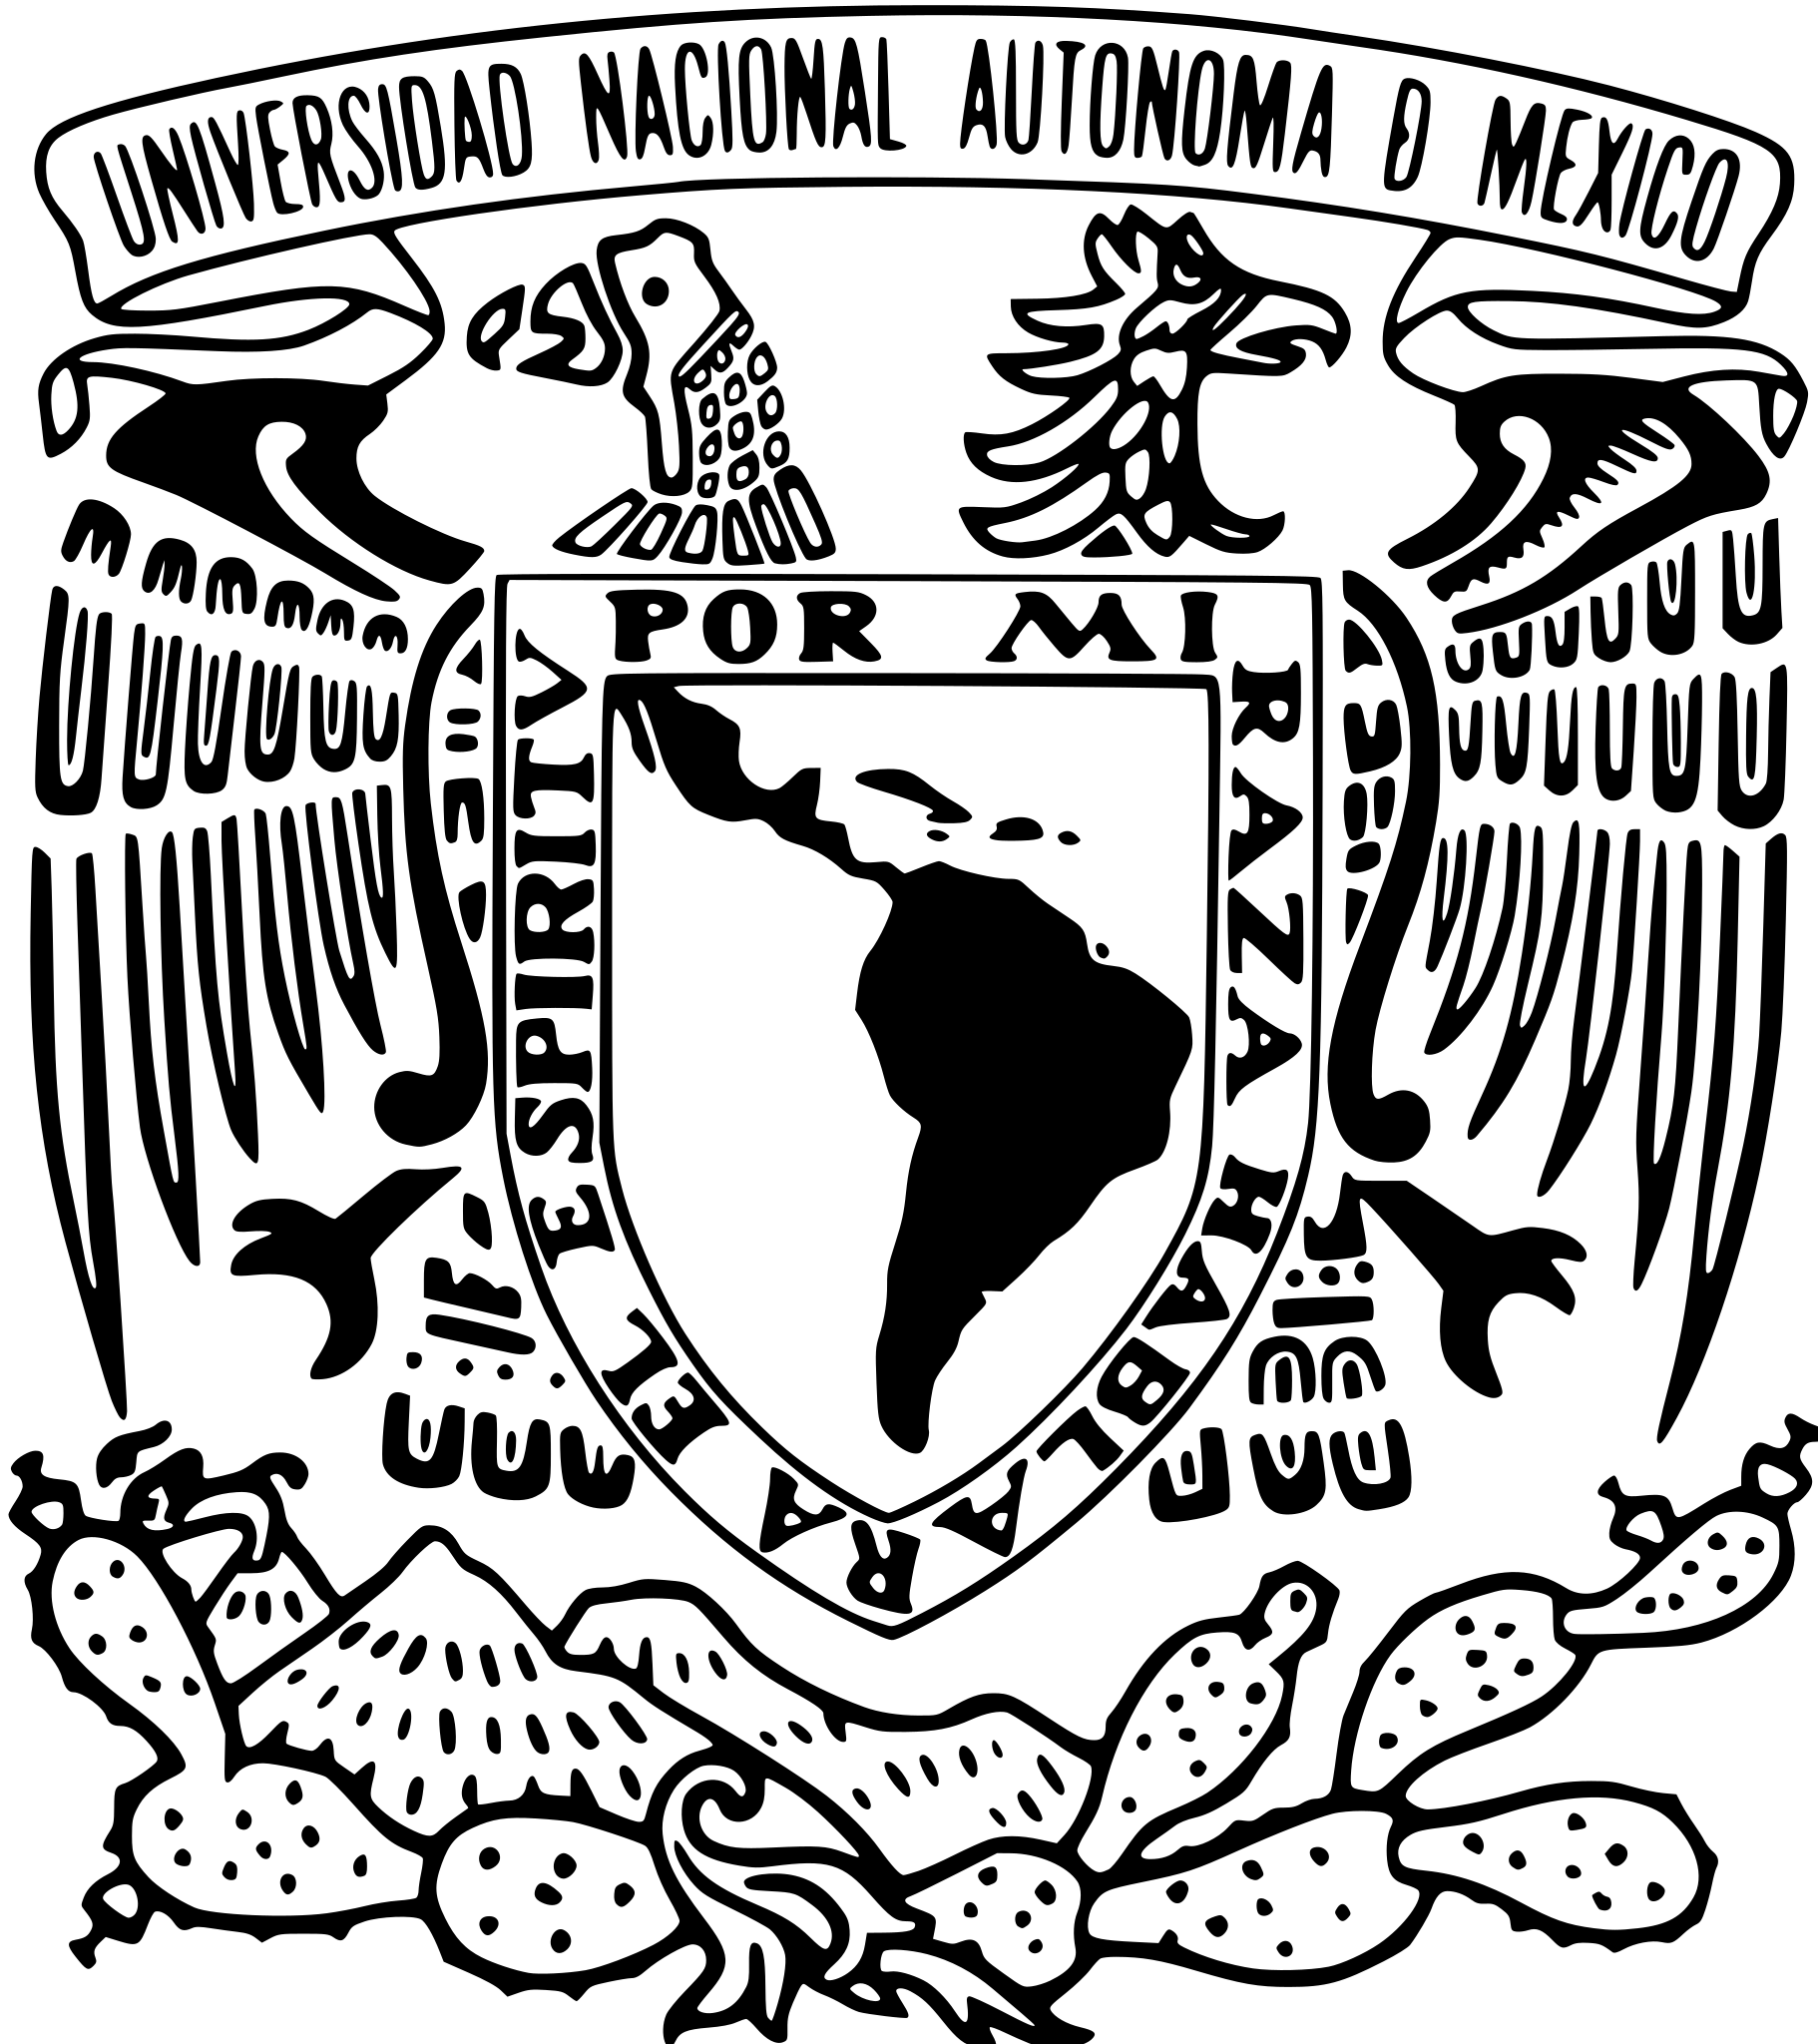
\includegraphics[width=1in]{EscudoUNAM.png}
       \end{flushright}
    \end{minipage}
    \begin{minipage}[H]{0.62 \textwidth}
        \begin{center}
            {\large \textsc{Universidad Nacional Autónoma de México}}
            \vspace{0.25cm}
            \\
            { \huge \textbf{Tarea 4}}
            \\
            \vspace{0.25cm}
            
            \textbf{Introducción a Ciencias de la Computación}
	   		\\
	        \vspace{0.25cm}
	        Rodrigo André Decuir Fuentes
            \vspace{0.2cm}
        \end{center}
        \vspace{0.05cm}
    \end{minipage}
    \begin{minipage}[t]{0.165 \textwidth}
        \begin{flushleft}
            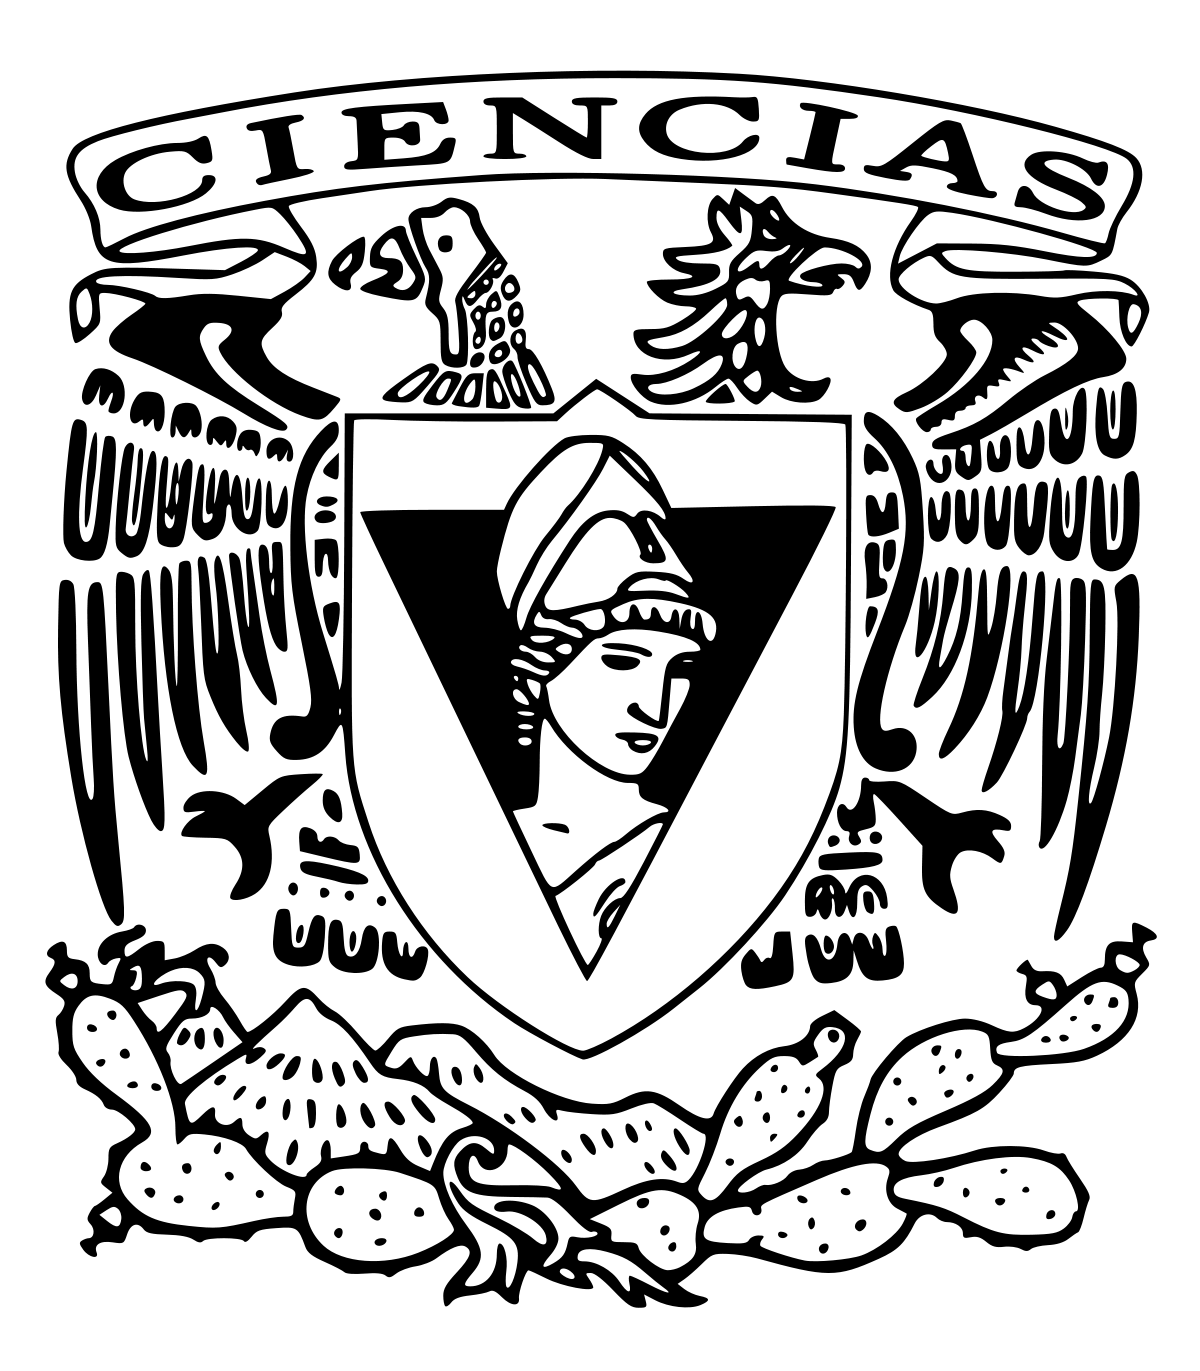
\includegraphics[width=1in]{Fciencias_UNAM.png}
        \end{flushleft}
    \end{minipage}
\begin{tikzpicture}
    \draw[thick] (-6.5,0)--(11.2,0);
\end{tikzpicture}
%%%%%%%%%%%%%%%%%%%%%%%%%%%%%%%%%%%%%%%%%%%%%%%%%%%%%%%%%
\section*{Teoría}
\subsection*{Responde las siguientes preguntas:}
    \begin{enumerate}
	    \item \textbf{¿En Java es posible la herencia múltiple? Justifica tu respuesta.}
            \begin{itemize}
                \item Java \textbf{no} soporta la herencia múltiple
                \item \textbf{Java solo soporta la herencia simple}, en donde cada clase se deriva sólo de una superclase
                      directa. Por otro lado, no soporta la herencia múltiple, que ocurre cuando una clase se 
                      deriva de más de una superclase directa.
            \end{itemize}
        \item \textbf{¿Por redefinir entiendes sobrecargar?}
            \begin{itemize}
                \item \textbf{No}, redefinir hace referencia a la \textit{sobrescritura de métodos}, la cual reutiliza
                      el código existente para modificar la forma de trabajar de un método sin modificar su firma. 
            \end{itemize}
        \item \textbf{¿Cuál es la finalidad de las Excepciones?}
            \begin{itemize}
                \item \textbf{Crear programas} tolerantes a fallas(\textbf{robustos}), que pueden resolver(o manejar) las excepciones.
                      En muchos casos, esto permite a un programa continuar su ejecución como si no hubiera encontrado
                      ningún problema. 
            \end{itemize}
        \item \textbf{Describe con tus propias palabras lo que indican las siguientes excepciones: }
            \begin{enumerate}
                \item \textbf{IllegalArgumentException.} 
                    \begin{itemize}
                        \item Para los valores fuera de rango, se lanza una excepción de tipo IllegalArgumentException,
                            la cual notifica que se \textbf{pasó un argumento inválido a un método}.  
                    \end{itemize}
                \item \textbf{IndexOutOfBoundsException.} 
                    \begin{itemize}
                        \item Cuando se ejecuta un programa en Java, se verifica la validez 
							  de los índices de los elementos del arreglo;
							  todos los índices deben ser mayores o iguales a 0 y menores que
                              la longitud del arreglo. Cualquier \textbf{intento de acceder a un elemento
                              fuera de} ese \textbf{rango de índices} produce un error en tiempo de ejecución,
							  el cual se conoce como ArrayIndexOutOfBoundsException. 
                    \end{itemize}
                \item \textbf{NullPointerException.} 
                    \begin{itemize}
                        \item Notifica sobre cualquier \textbf{intento de llamar} a un método sobre \textbf{una referencia null}. 
                    \end{itemize}
                \item \textbf{ArithmeticException.}
                    \begin{itemize}
                        \item Dicha excepción ocurre en el momento en que se proporciona al programa un valor
                            con \textbf{errores de aritmética}, por ej. dividir entre cero. La clase ArithmeticException
							  no necesita importarse, ya que se encuentra en el paquete java.lang 
                    \end{itemize}
            \end{enumerate}
        \item \textbf{¿Qué significa \textit{serializar} un objeto?}
            \begin{itemize}
                \item En principio quiere decir que se agrega el texto \textit{implements Serializable} al final
                      de la primera línea de la declaración de una clase. Pero el significado detrás de esto
                      es que se pueden \textbf{convertir objetos a representaciones de bytes que nos permitan guardarlos en serie}.
            \end{itemize}
        \item \textbf{Explica el término \textit{Persistencia}.}
            \begin{itemize}
                \item La persistencia es el \textbf{\textit{mecanismo} que se usa para persistir información de un determinado tipo
                    entre distintas ejecuciones del programa}. Nos permite almacenar, transferir y recuperar el estado
                      de los objetos, es decir, engloba el proceso de seriar(convertir objetos a representaciones de
                      bytes que nos permitan guardarlos en serie) y deseriar(convertir representaciones de bytes a objetos
                      que nos permitan cargarlos en serie).
            \end{itemize}
    \end{enumerate}
\end{document}
